\section{Digital Logic}

\subsection{Boolean Algebra}
First proposed by George Boole in 1854.
Variables in boolean algebra are always either 0 or 1.

\begin{definition}[Boolean Function]\label{def:boolean-function}
    A function in boolean algebra that takes $k$ variables is defined as:
    \begin{equation*}
        f: \{0,1\}^k \rightarrow \{0,1\}
    \end{equation*}
\end{definition}

\begin{definition}[Boolean Operations]
    In boolean algebra, the basic operations are denoted as follows:
    \begin{itemize}
        \item \textbf{AND}: $A\cdot B$ (or simply $AB$), gives 1 iff $A=B=1$;
        \item \textbf{OR}:  $A+B$, gives 1 if $A=1$ or $B=1$;
        \item \textbf{NOT}: $\overline{A}$, inverts the value of $A$;
        \item \textbf{NAND}: $\overline{A\cdot B}$, the complement of AND;
        \item \textbf{NOR}: $\overline{A+B}$, the complement of OR;
        \item \textbf{XOR}: $A\oplus B$, gives 1 iff one and only one of $A$ and $B$ is 1.
    \end{itemize}
\end{definition}

\begin{remark}
    $A\oplus B = \overline{A}B + A\overline{B}$;

    $\overline{A\oplus B} = \overline{\overline{A}B + A\overline{B}}
    = (\overline{\overline{A}B})(\overline{A\overline{B}}) = (A+\overline{B})(\overline{A}+B)
    = A\overline{A}+\overline{AB}+AB+B\overline{B} = AB+\overline{AB}$
\end{remark}

The truth tables of AND, OR, XOR, and NOT are given by:
\begin{table}[h]
\centering
\begin{tabular}{|c|c||c|c|c|c|}
    \hline
    $A$ & $B$ & $A\cdot B$ & $A+B$ & $A\oplus B$ & $\overline{A}$\\
    \hline
    0 & 0 & 0 & 0 & 0 & 1 \\
    0 & 1 & 0 & 1 & 1 & 1 \\
    1 & 0 & 0 & 1 & 1 & 0 \\
    1 & 1 & 1 & 1 & 0 & 0 \\
    \hline
\end{tabular}
\end{table}

\begin{definition}[Boolean Algebra Laws]\label{def:boolean-algebra-laws}
    The important laws of boolean algebra are:
    \begin{itemize}
        \item \textbf{Commutative Law}: $A+B = B+A$, $A\cdot B = B\cdot A$;
        \item \textbf{Identity Elements}: $A+0 = A$, $A\cdot 1 = A$;
        \item \textbf{Null Law}: $A+1 = 1$, $A\cdot 0 = 0$;
        \item \textbf{Idempotent Law}: $A+A = A$, $A\cdot A = A$;
        \item \textbf{Inverse Law}: $A+\overline{A} = 1$, $A\cdot\overline{A} = 0$;
        \item \textbf{Associative Law}: $(A+B)+C = A+(B+C)$, $(A\cdot B)\cdot C = A\cdot(B\cdot C)$;
        \item \textbf{Distributive Law}: $A\cdot(B+C) = A\cdot B + A\cdot C$, $A+(B\cdot C) = (A+B)\cdot(A+C)$;
    \end{itemize}
\end{definition}

\begin{proof}[Proof of Distributive Law $A+(B\cdot C) = (A+B)\cdot(A+C)$]
    \begin{align*}
        A+(B\cdot C) &= A\cdot A + A\cdot C + B\cdot A + B\cdot C
    \end{align*}
    Suppose $A=1$, then the equation becomes:
    \begin{align*}
        1+(B\cdot C) &= 1\cdot 1 + 1\cdot C + B\cdot 1 + B\cdot C\\
        1 &= 1 + C + B + B\cdot C\\
        1 &= 1 + B\cdot C
    \end{align*}
    which is true by the Null Law. Now, suppose $A=0$, then the equation becomes:
    \begin{align*}
        0+(B\cdot C) &= 0\cdot 0 + 0\cdot C + B\cdot 0 + B\cdot C\\
        B\cdot C &= 0 + 0 + 0 + B\cdot C\\
        B\cdot C &= B\cdot C
    \end{align*}
    which is true by the Idempotent Law.
\end{proof}

\begin{theorem}[De Morgan's Theorem]\label{def:de-morgans-theorem}
    De Morgan's Theorem states that:
    \begin{align*}
        \overline{A+B} &= \overline{A}\cdot\overline{B}\\
        \overline{A\cdot B} &= \overline{A}+\overline{B}
    \end{align*}

    More generally, we have:
    \begin{align*}
        \overline{A+B+\dots+N} &= \overline{A}\cdot\overline{B}\cdot\dots\cdot\overline{N}\\
        \overline{AB\dots N} &= \overline{A}+\overline{B}+\dots+\overline{N}
    \end{align*}
\end{theorem}

\subsubsection{Logic Gates}

Other than expressions, boolean algebra can also be implemented using logic gates.
Below is a list of the corresponding gates for the basic boolean operations:

\begin{center}
    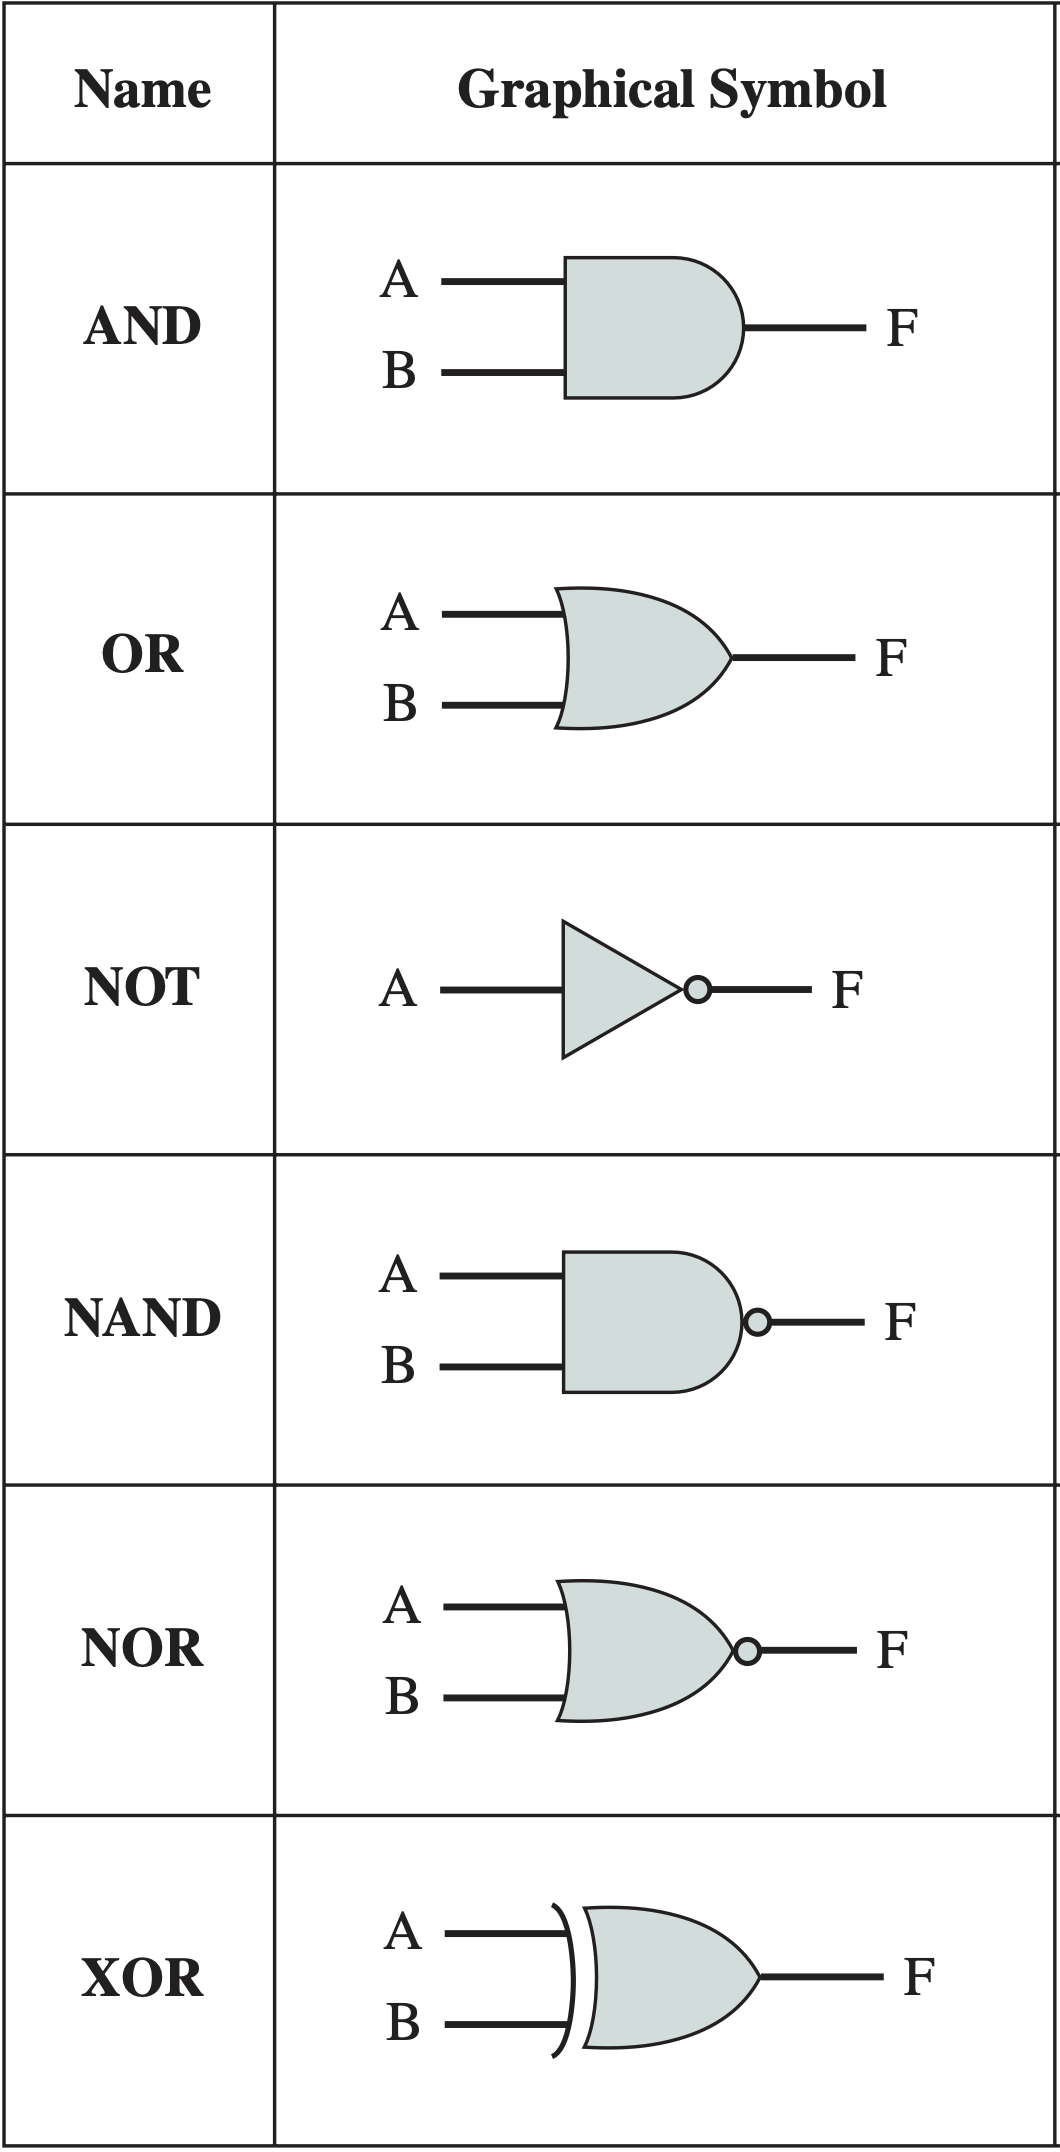
\includegraphics[scale=0.3]{chaps/digital-logic/logic-gates.png}
\end{center}

\subsection{Functional Completeness}\label{subsec:functional-completeness}
\begin{definition}[Functional Completeness]
    A set of logic gates is said to be functionally complete if any boolean function
    can be implemented using only gates from that set.
\end{definition}

\subsubsection{The \texttt{AND}, \texttt{OR}, \texttt{NOT} Set}

The set of \texttt{AND}, \texttt{OR}, and \texttt{NOT} gates is functionally complete,
i.e. they can be used to create any arbitrary boolean function.

\subsubsection{The \texttt{AND}, \texttt{NOT} Set}

By using De Morgan's Theorem, the OR operation can be implemented using only
AND and NOT gates. Therefore, this reduced set is itself functionally
complete. We start with the NAND expression in De Morgan's Theorem:
\begin{align*}
    \overline{A+B} &= \overline{A}\cdot\overline{B} \\
    \intertext{Then, we apply the NOT operation to both sides:}
    \overline{\overline{A+B}} &= \overline{\overline{A}\cdot\overline{B}} \\
    A + B &= \overline{\overline{A}\cdot\overline{B}}
\end{align*}
The left hand side is exactly the OR operation, implemented using only AND and NOT gates.

\subsubsection{The \texttt{OR}, \texttt{NOT} Set}

Similarly, by using De Morgan's Theorem, the AND operation can be implemented using only
OR and NOT gates. Therefore, this reduced set is itself functionally complete.

\subsubsection{The \texttt{NAND} Set}

The NAND operation alone can also be used to implement the AND, OR, and NOT operations.
By applying NAND between $A$ and $A$ itself, we have:
\begin{equation*}
    \overline{A\cdot A} = \overline{A} \text{ (NOT operation)}
\end{equation*}

Similarly, by applying NAND over the value of $\overline{A\cdot B}$, we have $A\cdot B$,
which is the AND operation.

Finally, by applying NAND between $\overline{A}$ and $\overline{B}$
(i.e. $\overline{\overline{A}\cdot\overline{B}}$), according to
De Morgan's Theorem, we have $A+B$, which is the OR operation.

Since AND, OR, and NOT operations can be implemented using only NAND gates,
and the set of AND, OR, and NOT gates is functionally complete, the NAND set is also
functionally complete.

\subsubsection{The \texttt{NOR} Set}

Similar to the NAND set, the NOR set is also functionally complete.

\subsection{Implementation of Boolean Functions}

Suppose we would like to implement a boolean function $F(A, B, C)$ with the following
truth table:

\begin{table}[h]
\centering
\begin{tabular}{|c|c|c||c|}
    \hline
    $A$ & $B$ & $C$ & $F(A, B, C)$ \\
    \hline
    0 & 0 & 0 & 0 \\
    0 & 0 & 1 & 0 \\
    0 & 1 & 0 & 1 \\
    0 & 1 & 1 & 1 \\
    1 & 0 & 0 & 0 \\
    1 & 0 & 1 & 0 \\
    1 & 1 & 0 & 1 \\
    1 & 1 & 1 & 0 \\
    \hline
\end{tabular}
\end{table}
The technique is to use either the Sum-of-Products (SOP) or the Product-of-Sums (POS) method.

\subsubsection{Sum-of-Products (SOP)}

SOP usually has the form of $F = XYZ + XYZ + \dots$, every term should be the product
of all the variables, appearing exactly once. Such terms are named ``minterms''.
To implement the function $F$, first identify the rows in the truth table where $F=1$,
then for each row, construct the minterm by taking the product of all the variables,
such that the sum of the minterms will give 1.

\begin{example}
    From the truth table, we observe that $F=1$ on the 3rd, 4th, and 7th rows.
    
    For the 3rd row, the product $\overline{A}B\overline{C}$ equals 1.

    For the 4th row, the product $\overline{A}BC$ equals 1.

    For the 7th row, the product $AB\overline{C}$ equals 1.

    Therefore, the function $F$ can be implemented as:
    \begin{equation*}
        F = \overline{A}B\overline{C} + \overline{A}BC + AB\overline{C}
    \end{equation*}
\end{example}

This method works because:
\begin{itemize}
    \item any other input combinations will make all the minterms 0, and the sum of 0's is 0;
    \item when one of the minterms is 1, the sum will be 1.
\end{itemize}

\subsubsection{Product-of-Sums (POS)}

Contrast to SOP, POS usually has the form of $F = (X+Y+Z)(X+Y+Z)\dots$.
The approach is to identify the rows in the truth table where $F=0$,
then for each row, construct a \textbf{product} (NOT sum) of all the variables,
such that the term give 1, then apply a NOT operation on the product. Connect all the terms
together with AND operators, and simplify using De Morgan's Theorem.

\begin{example}
    From the truth table, we observe that $F=0$ on rows other than the 3rd, 4th, and 7th.

    For the 1st row, we construct the product
    $\overline{\overline{A}\cdot\overline{B}\cdot\overline{C}}$, which equals 0.

    For the 2nd row, we construct the product
    $\overline{\overline{A}\cdot\overline{B}\cdot C}$, which equals 0.

    $\dots$

    For the 8th row, we construct the product
    $\overline{A\cdot B\cdot C}$, which equals 0.

    Then, connect the terms together with AND operations, we have:
    \begin{equation*}
        F = \left(\overline{\overline{A}\,\overline{B}\,\overline C }\right) \cdot 
            \left(\overline{\overline{A}\,\overline{B}\,          C }\right) \cdot 
            \left(\overline{          A \,\overline{B}\,\overline{C}}\right) \cdot 
            \left(\overline{          A \,\overline{B}\,          C }\right) \cdot
            \left(\overline{          A \,          B \,          C }\right)
    \end{equation*}

    For each product, apply De Morgan's Theorem
    $\overline{ABC} = \overline{A} + \overline{B} + \overline{C}$ to simplify, we have:
    \begin{equation*}
        F = (A+B+C)\cdot
            (A+B+\overline{C})\cdot
            (\overline{A}+B+C)\cdot
            (\overline{A}+B+\overline{C})\cdot
            (\overline{A}+\overline{B}+\overline{C})
    \end{equation*}
\end{example}

\begin{remark}
    Whether to use SOP or POS depends on the truth table. Generally, when there are
    less 1's in the truth table, it is easier to use SOP. When there are less 0's,
    it is easier to use POS.
\end{remark}

\subsubsection{Simplification by Boolean Algebra}

After constructing the SOP or POS expression, it is possible to simplify the expression
using the laws of boolean algebra.

\begin{example}
    The $F$ we have implemented using SOP can be simplified as follows:
\begin{align*}
    F &= \overline{A}B\overline{C} + \overline{A}BC + AB\overline{C} \\
      &= \overline{A}B\overline{C} + \overline{A}BC + \overline{A}B\overline{C} + AB\overline{C} \\
      &= \overline{A}B \left(\overline{C} + C\right) + \left(\overline{A} + A\right) B\overline{C} \\
      &= \overline{A}B + B\overline{C}
\end{align*}
\end{example}

\subsubsection{Simplification by Karnaugh Maps}

For boolean expressions with two to four variables, construct Karnaugh maps to simplify
the expression. Rule for rows and columns: adjacent rows/columns must differ by only one variable.
Rules for grouping 1's: each group-
\begin{itemize}
    \item should be as large as possible;
    \item must be rectangular in shape;
    \item must contain number of 1's that is a power of 2 (1, 2, 4, 8, etc.);
    \item can overlap or wrap around the edges;
    \item should contain at least one 1 that is not in any other groups.
\end{itemize}

\begin{example}
    To simplify $F = \overline{A}B\overline{C} + \overline{A}BC + AB\overline{C}$,
    construct the map:

    
    \begin{center}
    \begin{tabular}{rrcccc}
                                            &                                   & \multicolumn{4}{c}{\textbf{BC}}                                                                                       \\
                                            &                                   & \textbf{00}                       & \textbf{01}               & \textbf{11}               & \textbf{10}               \\ \cline{3-6} 
        \multirow{2}{*}{\textbf{A}}         & \multicolumn{1}{r|}{\textbf{0}}   & \multicolumn{1}{c|}{}             & \multicolumn{1}{c|}{}     & \multicolumn{1}{c|}{\color[HTML]{FF0000}1}    & \multicolumn{1}{c|}{\color[HTML]{6200c9}1}    \\ \cline{3-6} 
                                            & \multicolumn{1}{r|}{\textbf{1}}   & \multicolumn{1}{c|}{}             & \multicolumn{1}{c|}{}     & \multicolumn{1}{c|}{}     & \multicolumn{1}{c|}{\color[HTML]{0000FF}1}    \\ \cline{3-6} 
    \end{tabular}
    \end{center}
    
    They can be separated into two groups - one {\color[HTML]{FF0000}horizontal} and one {\color[HTML]{0000FF}vertical}.
    For the horizontal group, observe that regardless of the value of $C$, the value of $F$
    is always one, implying an expression of $\overline{A}B$. For the vertical group,
    the value of $F$ is always one regardless of the value of $A$, implying an expression of
    $B\overline{C}$. Therefore, the simplified expression is $\overline{A}B + B\overline{C}$.
\end{example}

\subsubsection{Application: Multiplexer}

\begin{example}
    Suppose we have a 2-to-1 multiplexer $s$ defined as:
    \begin{equation*}
        s = \begin{cases}
            a & \text{if } t=0 \\
            b & \text{if } t=1
        \end{cases}
    \end{equation*}
    The logical expression of the multiplexer is in fact $s = f(a, b, t)$.
    To solve for the expression, write down the truth table, and apply either SOP or POS
    to simplify the expression.
\end{example}

\subsection{Adders}

Adders can be created using logic gates. When they are chained together, they can be used
to perform addition of binary numbers. There are two types of adders:
\begin{itemize}
    \item \textbf{Half Adder}: adds two bits together, produce a sum and a carry (2-in-2-out);
    \item \textbf{Full Adder}: adds two bits and a carry produced from the previous addition,
                                produce a sum and a carry (3-in-2-out).
\end{itemize}

\subsubsection{Half Adder}

Consider the truth table of adding two digits $A$ and $B$:
\begin{table}[h]
\centering
\begin{tabular}{|c|c||c|c|}
    \hline
    $A$ & $B$ & Sum ($S$) & Carry ($C$) \\
    \hline
    0 & 0 & 0 & 0 \\
    0 & 1 & 1 & 0 \\
    1 & 0 & 1 & 0 \\
    1 & 1 & 0 & 1 \\
    \hline
\end{tabular}
\end{table}

We can observe that $S=A\oplus B$ and $C=A\cdot B$. However, the half adder cannot be used
to add numbers with more than one digit, because it does not take into account the carry
from the previous addition.

\subsubsection{Full Adder}

Now take into account the carry from the previous addition ($C'$), we have the following truth table:
\begin{table}[h]
\centering
\begin{tabular}{|c|c|c||c|c|}
    \hline
    $A$ & $B$ & $C'$ & Sum ($S$) & Carry ($C$) \\
    \hline
    0 & 0 & 0 & 0 & 0 \\
    0 & 0 & 1 & 1 & 0 \\
    0 & 1 & 0 & 1 & 0 \\
    1 & 0 & 0 & 1 & 0 \\
    1 & 1 & 0 & 0 & 1 \\
    0 & 1 & 1 & 0 & 1 \\
    1 & 0 & 1 & 0 & 1 \\
    1 & 1 & 1 & 1 & 1 \\
    \hline
\end{tabular}
\end{table}

Apply SOP, we have:
\begin{align*}
    S &= \overline{A}\overline{B}C' + \overline{A}B\overline{C'} + A\overline{B}\overline{C'} + ABC' \\
      &= C'(\overline{A}\overline{B} + AB) + \overline{C'}(\overline{A}B + A\overline{B}) \\
      &= C'(\overline{A\oplus B}) + \overline{C'}(A\oplus B) \\
      &= C'\oplus(A\oplus B)
\end{align*}
and
\begin{align*}
    C &= AB\overline{C'} + \overline{A}BC' + A\overline{B}C' + ABC' \\
      &= AB(\overline{C'} + C') + C' (\overline{A}B + A\overline{B}) \\
      &= AB + C'(A\oplus B)
\end{align*}